\documentclass{article}
\usepackage[dvipsnames]{xcolor}
\usepackage[paperwidth=20cm, paperheight=4.5cm, margin = 0cm, top=1.75cm]{geometry}

\usepackage{amsmath}
\usepackage{pgf}
\usepackage{tikz}
\usetikzlibrary{arrows,automata}

\tikzstyle{source}  = [draw,circle,fill=black,thick,inner sep=0mm,minimum size=2mm]

\begin{document}
\begin{center}
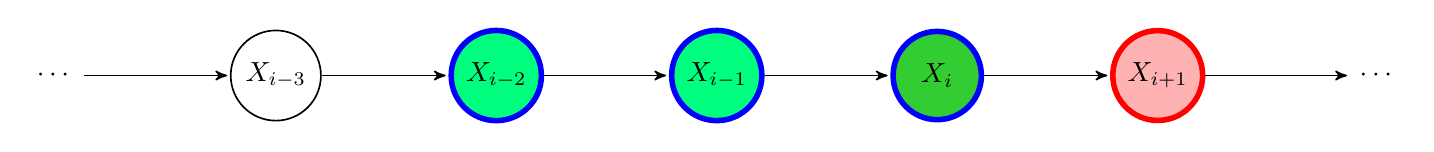
\begin{tikzpicture}[->,>=stealth',shorten >=1pt,auto,node distance=2.8cm,semithick]
                    
\node        (X0) {$\cdots$}; 
\node[state] (X1) [right of=X0] {$X_{i-3}$}; 
\node[state, fill=SpringGreen, draw=blue, line width=2pt] (X2) [right of=X1] {$X_{i-2}$};                   
\node[state, fill=SpringGreen, draw=blue, line width=2pt] (X3) [right of=X2] {$X_{i-1}$};                   
\node[state, fill=LimeGreen, draw=blue, line width=2pt] (X4) [right of=X3] {$\hspace{0.5em}X_{i}\hspace{0.5em}$};                   
\node[state] (X5) [right of=X4, fill=red, 
opacity = 0.3, draw opacity=1,  draw=red, line width=2pt, text opacity =1] {$X_{i+1}$};                   
\node        (X6) [right of=X5] {$\cdots$};                   

\path
    (X0) edge node {} (X1)  
	(X1) edge node {} (X2)
	(X2) edge node {} (X3)
	(X3) edge node {} (X4)
	(X4) edge node {} (X5)
	(X5) edge node {} (X6);

\end{tikzpicture}
\end{center}

\end{document}
